\documentclass[12pt]{report}
\usepackage[utf8]{inputenc}
\usepackage[margin=1.2in]{geometry}
\usepackage{graphicx}
\usepackage{float}
\usepackage{subcaption}
\usepackage{amsmath}
\usepackage{amssymb}
\usepackage{ulem}
\usepackage{bm}
\usepackage{framed}
\usepackage{xcolor}
\usepackage{ragged2e}
\usepackage{color}
\usepackage{soul}
\usepackage{cancel}
\graphicspath{ {images/} }
\setlength{\parskip}{1em}
\allowdisplaybreaks


\usepackage{titling}
\newcommand{\subtitle}[1]{%
	\posttitle{%
		\par\end{center}
	\begin{center}\large#1\end{center}
	\vskip0.5em}%
}

\newenvironment{blueframed}[1][blue]
{\def\FrameCommand{\fboxsep=\FrameSep\fcolorbox{#1}{white}}%
	\MakeFramed {\advance\hsize-\width \FrameRestore}}
{\endMakeFramed}

\title{Tutorial 1}
\subtitle
{
	\textbf{keywords}: EViews, variables, data set, sample, population, descriptive analytics, summary statistics, histogram, scatter plots, correlation, simple linear regression model, predictive analytics
	
	\textbf{estimated reading time}: 19 minutes
}
\author{Quang Bui}
\date{July 24, 2018}

\begin{document}
	
	\maketitle

	\section*{Question 1}
	\underline{Exploring EViews with \textit{wine.wf1}}
	
	\noindent EViews is a computer software designed specifically for econometric analysis. In today's class, we use EViews to perform basic econometric analysis on the workfile, $wine.wf1$.
		\begin{figure}[H]
			\centering
			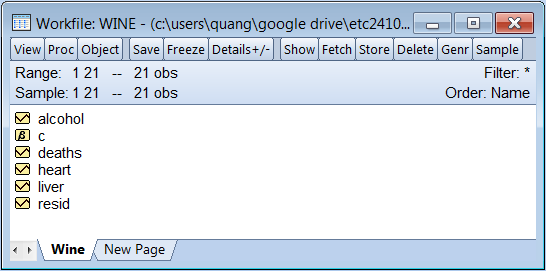
\includegraphics{ss1}
		\end{figure}
		\vspace{-\baselineskip}
		\noindent \textbf{Objects}
		
		\noindent The elements in the whitespace of the \textit{wine.wf1} workfile are called EViews \textbf{objects}. There are many types of EViews objects but in this unit we mostly focus on \textbf{series}, \textbf{groups}, \textbf{graphs}, \textbf{equations}, \textbf{scalar} and \textbf{coef} objects. Each object type is identified by a unique icon,
		\vspace{-\baselineskip}
		\begin{center}
			\begin{tabular}{ c c}
				\textbf{Icon} & \textbf{Object} \\
				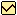
\includegraphics{series} & series \\
				
\includegraphics{group} & group \\
				
\includegraphics{graph} & graph \\
				
\includegraphics{equation} & equation \\
				
\includegraphics{scalar} & scalar \\
				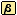
\includegraphics{coef} & coef \\
			\end{tabular}
		\end{center}
		\vspace{-\baselineskip}
		%Title: Data set
		\newpage	
		\noindent \textbf{Data set}
		\begin{figure}[H]
			\centering
			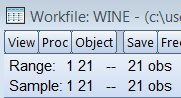
\includegraphics{dataset1}
		\end{figure}
		\vspace{-\baselineskip}
		\begin{itemize}
			\item \textit{Range: 1 21 -- 21 obs} indicates that the data set in \textit{wine.wf1} contains 21 observations starting at observation number 1 to 21.
			\item \textit{Sample: 1 21 -- 21 obs} denotes the sample which EViews will use to produce graphs, run regressions, and obtain other EViews outputs. The current sample contains all observations in the data set.
		\end{itemize}
		\noindent \textbf{Variables} \par
			\noindent The \textit{wine.wf1} workfile contains data on 21 countries. This data set holds information about each country through the following variables:
			\vspace{-\baselineskip}
			\begin{itemize}
				\item \textit{alcohol} - litres of wine consumed per capita per annum
				\item \textit{deaths} - number of deaths per 100,000 of population
				\item \textit{heart} - number of deaths from heart disease per 100,000 of population
				\item \textit{liver} - number of deaths from liver disease per 100,000 of population
			\end{itemize}
			\vspace{-\baselineskip}
			\noindent A description of each variable appears by clicking \textbf{Details +/-} on the workfile windows.
			
			\begin{figure}[H]
				\centering
				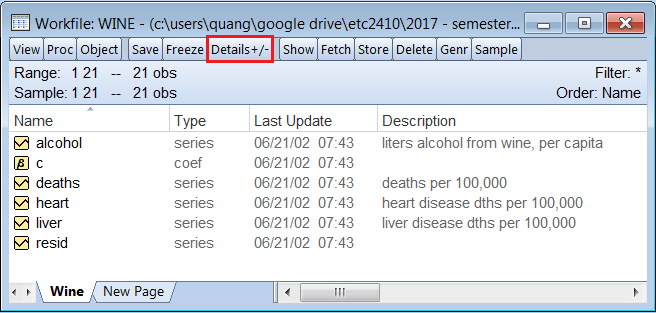
\includegraphics[width = 1\textwidth]{wf1}
			\end{figure}
			\vspace{-\baselineskip}
			\noindent
			To view the data in a single variable, double click the variable. To view the data in multiple variables, select and highlight the variables of interest then,
			$$Right\ click \to Open \to as\ Group$$
			\begin{figure}[H]
				\centering
				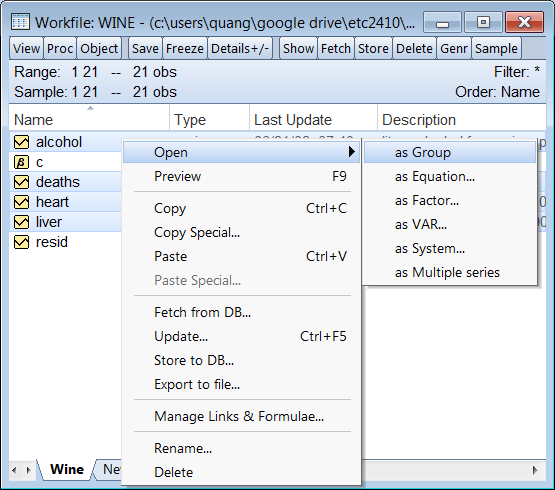
\includegraphics[width=0.67\textwidth]{group1}
				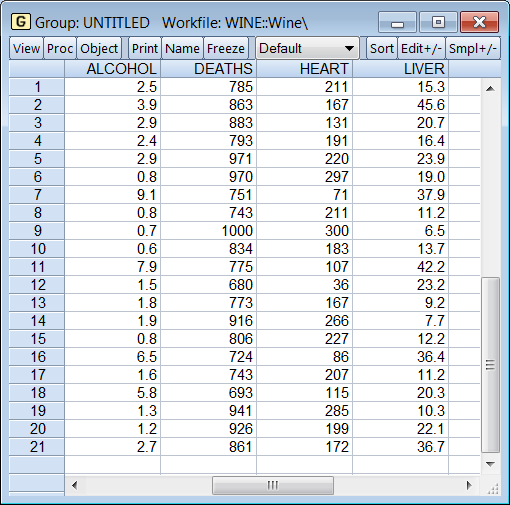
\includegraphics[width=0.67\textwidth]{group2}
			\end{figure}
	\newpage	
	\section*{Question 2}
	\underline{Descriptive analytics with histograms and descriptive statistics}	
		
		\noindent To obtain the histogram and descriptive statistics of the variable \textit{alcohol}, 
		\begin{figure}[H]
			\centering
			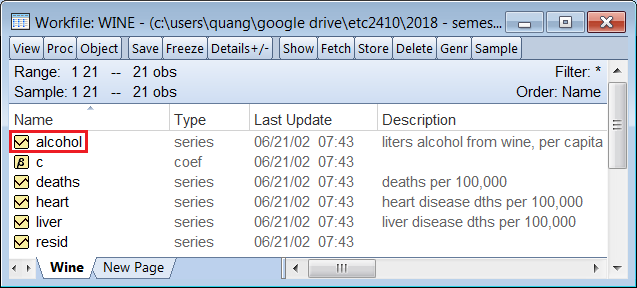
\includegraphics{q2_1}
		\end{figure} \vspace{-\baselineskip}
		\justify		
		\noindent double-click on the variable \textit{alcohol},
		
		\begin{figure}[H]
			\centering
			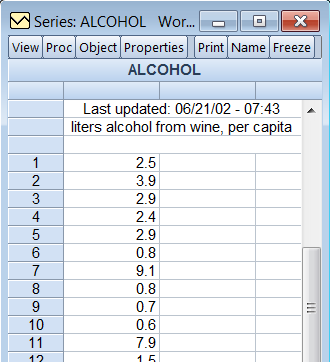
\includegraphics{alcohol}
		\end{figure} \vspace{-\baselineskip}
		\justify
		\noindent then,
		$$View \to Descriptive\ Statistics \And Tests \to Histogram\ and\ Stats$$
		
		\begin{figure}[H]
			\centerline{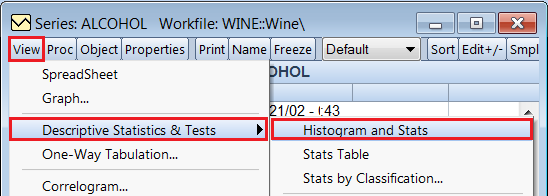
\includegraphics{alcohol1}}
		\end{figure}
		\vspace{-\baselineskip}
		\begin{figure}[H]
			\centerline{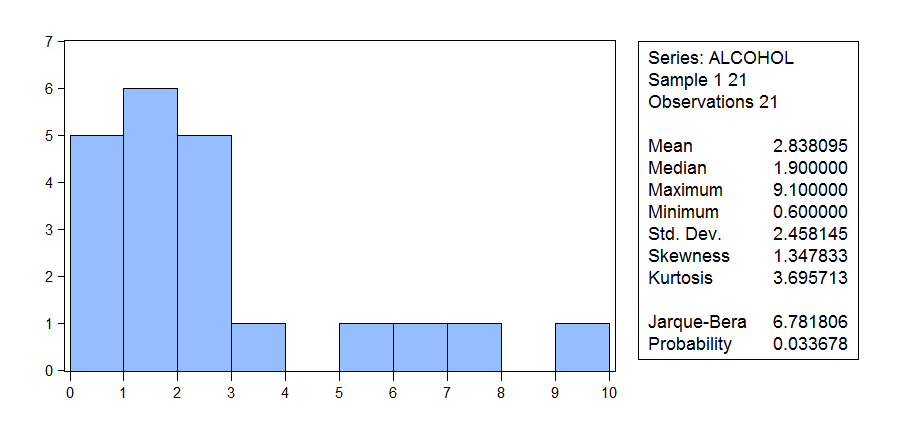
\includegraphics{alcohol2}}
			\caption{Histogram and descriptive statistics of litres of wine consumed per capita per annum from a sample of 21 countries.}
			\label{fig:hist1}
		\end{figure}
		\vspace{-\baselineskip}
		\noindent As we can see from Figure \ref{fig:hist1}, wine consumption per capita per annum is positively skewed (right-tailed). On average, countries consume approximately 2.838 litres of wine per capita per annum. The mean wine consumption is greater than the median wine consumption, $$2.838 > 1.90$$ which also indicates that wine consumption is positively skewed. \par
		\newpage
		\noindent We can also obtain descriptive statistics for multiple variables in a single spreadsheet. One way to do this is by selecting \textit{Quick} from the EViews workfile menu,
		$$Quick \to Group\ Statistics \to Descriptive\ Statistics \to Common\ sample$$
		\begin{figure}[H]
			\centerline{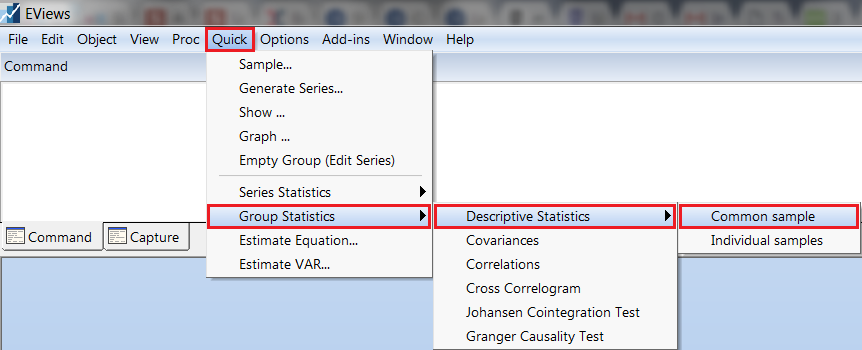
\includegraphics{q2_2}}
		\end{figure}
		\vspace{-\baselineskip}
		\noindent then type in the variables of interest into the \textit{Series List} window,
		\begin{figure}[H]
			\centerline{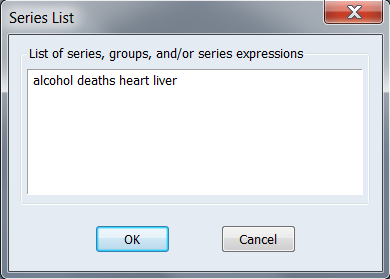
\includegraphics{q2_3}}
		\end{figure}		
		\vspace{-\baselineskip}
		\begin{figure}[H]
			\centerline{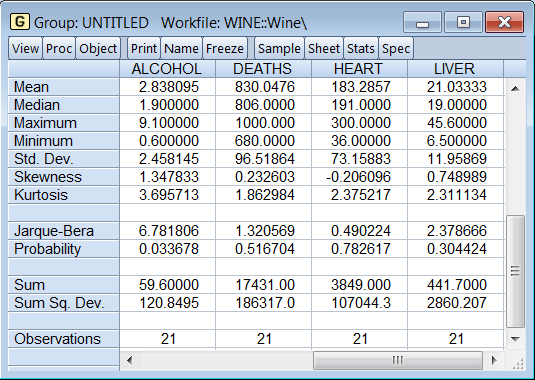
\includegraphics{dstat2}}
		\end{figure}	
		\vspace{-\baselineskip}
		\noindent Note: The \textit{Freeze} button takes a screenshot, while the \textit{Name} button names and saves the object into the workfile.

	\newpage	
	\section*{Question 3}
	\underline{Scatter plots and correlations}
		
		\noindent Scatter plots are graphs used to visually explore the relationship between two variables. To obtain a scatterplot of $deaths$ (y-axis) against $alcohol$ (x-axis),
		$$Quick \to Graph \dots$$
		\begin{figure}[H]
			\centerline{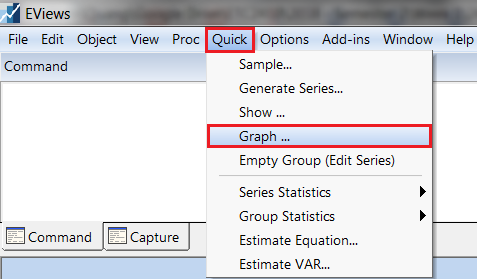
\includegraphics{q3_1}}
		\end{figure}
		\vspace{-\baselineskip}
		\noindent in the \textit{Series List} window, type the x-variable followed by the y-variable,
		\begin{figure}[H]
			\centerline{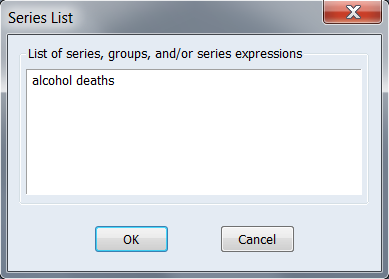
\includegraphics{q3_2}}
		\end{figure}
		\vspace{-\baselineskip}	
		\noindent Under \textit{Specific}, select \textit{Scatter} and press \textit{OK},
		$$Specific:Scatter \to OK$$
		\begin{figure}[H]
			\centerline{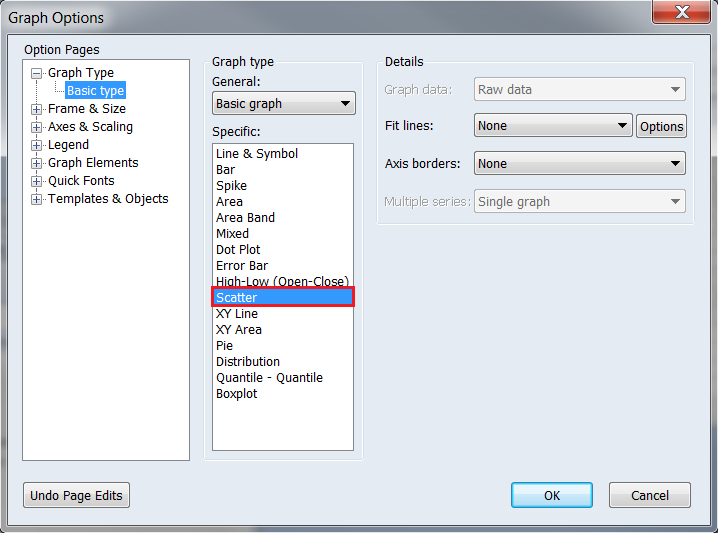
\includegraphics{scat3}}
		\end{figure}
		\vspace{-\baselineskip}	
		\noindent To give this graph the name \textit{scatter\_alcohol\_deaths}, select $Name$,
		\begin{figure}[H]
			\centerline{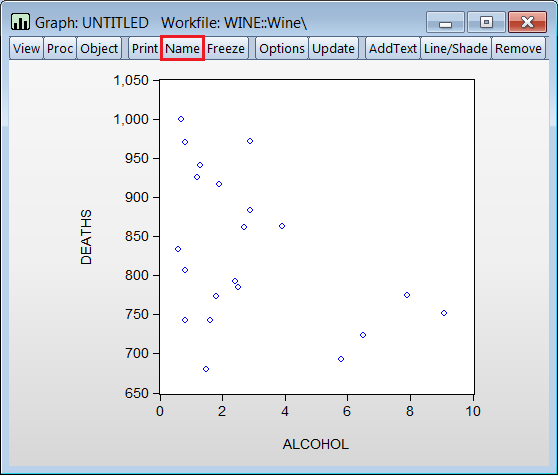
\includegraphics[width=0.7\textwidth]{q3_3}}
		\end{figure}
		\vspace{-\baselineskip}	
		then, $$Name\ to\ identify\ object:scatter\_alcohol\_deaths$$
		\begin{figure}[H]
			\centering
			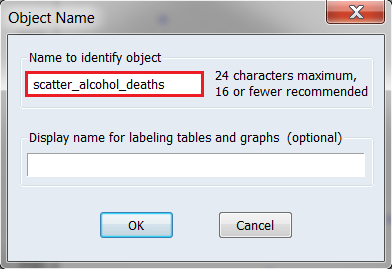
\includegraphics{name1}
		\end{figure}
		\vspace{-\baselineskip}	
		\begin{figure}[H]
			\centerline{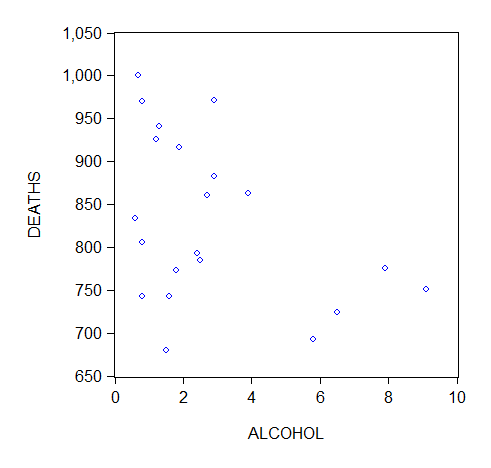
\includegraphics{scatter_alcohol_deaths}}
			\caption{Scatter plot of deaths per 100,000 of population against litres of wine consumption per capita per annum.}
			\label{fig:scat1}
		\end{figure}
		\vspace{-\baselineskip}	
		\noindent From the scatter plot, we observe a moderate negative linear relationship between wine consumption per capita per annum and  deaths per 100,000 of population. \par
		\newpage
		\noindent To obtain a table of sample correlation coefficients,
		$$Quick \to Group\ Statistics \to Correlations$$
		
		\begin{figure}[H]
			\centerline{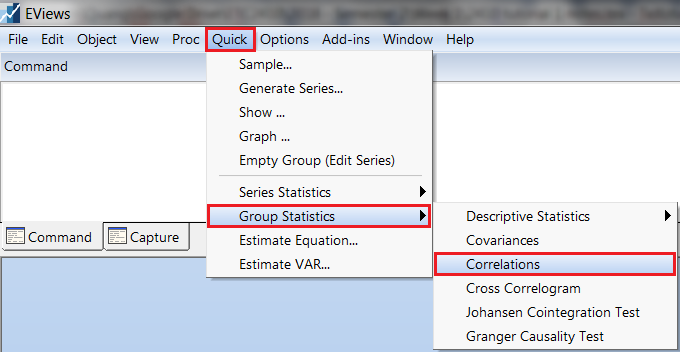
\includegraphics{q3_4}}
		\end{figure}		
		\vspace{-\baselineskip}		
		\noindent then type in the variables of interest into the \textit{Series List} windows,
		\begin{figure}[H]
			\centerline{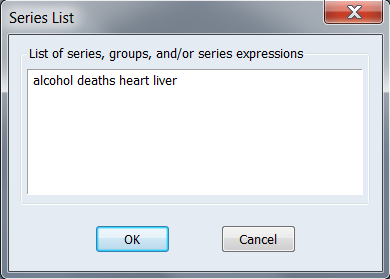
\includegraphics{q2_3}}
		\end{figure}		
		\vspace{-\baselineskip}	
		\begin{figure}[H]
			\centering
			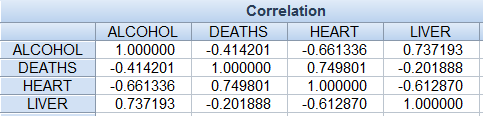
\includegraphics{corr2}
		\end{figure}
		\vspace{-\baselineskip}
		\newpage
		\noindent The numbers in the table above represent the following sample correlation coefficients:
		\begin{align*}
			&\widehat{corr}(alcohol,deaths) = -0.41420 \\
			% why does alcohol and death have a negative relationship? Here we have a numerical measure of the relationship between a country's wine consumption and their death rate but this relationship does not control for other factors which impact a country's death rate. It is quite reasonable to think of countries with high wine consumption levels to also be those with high average income levels and better overall living standards. As such, wine consumption could be representing or proxying for a country's wealth and wellness, which would explain why wine consumption and death rate have a negative relationship.
			&\widehat{corr}(alcohol,heart) = -0.66134 \\
			&\widehat{corr}(alcohol,liver) = 0.73719 \\
			&\widehat{corr}(deaths,heart) = 0.74980 \\
			% countries with high total death rate tend to have a high heart disease related death rate
			&\widehat{corr}(deaths,liver) = -0.20189 \\
		\end{align*}
		\noindent The sample correlation coefficient measures strength and direction of the linear relationship between 2 variables and takes on a value between -1 and 1. \begin{itemize}
			\item If the sample correlation coefficient equal to -1, then the two variables have a perfect negative linear relationship.
			\item If the sample correlation coefficient equal to 1, then the two variables have a perfect positive linear relationship.
			\item If the sample correlation coefficient equal to 0, then the two variables have no linear relationship.
		\end{itemize} Therefore, the magnitude of the sample correlation coefficient measures the strength of the linear relationship between two variables and the size of the sample correlation coefficient measures the direction of the linear relationship.
	\newpage	
	\section*{Question 4}
	\underline{Estimating a simple linear regression model}
		
		\justify
		\begin{blueframed}
			\textcolor{blue}{\textbf{Background}}
			\vspace{-\baselineskip}
			\justify
			\textcolor{blue}{\underline{Simple Linear Regression Model}}
			
			\noindent \textcolor{blue}
			{
				\noindent Simple - one independent variable \\
				Linear - linear in the parameters
			}	
		
			\noindent \textcolor{blue}
			{
				\noindent Suppose we specify a simple linear regression model of \textit{y} on a constant (intercept) and \textit{x},
				\begin{equation}
					y = \beta_0 + \beta_1x + u \label{eq:1}
				\end{equation}
				where \textit{u} is the error term that captures unobserved factors that affect \textit{y} (factors other than \textit{x} that affect $y$). It is included in the model because no matter how we specify the model, we cannot guarantee that the $x$ input will perfectly output $y$ i.e. there will always be some error. $\beta_0$ and $\beta_1$ are the intercept and slope coefficients respectively. They are population parameters and are unknown in practice.
			}
		
		\noindent \textcolor{blue}
			{	
				\noindent To quantify the relationship between $y$ and $x$, we need to estimate these population parameters. With data on \textit{y} and \textit{x}, we can use an estimator (more on this in subsequent weeks) to estimate (\ref{eq:1}), giving us estimates of $\beta_0$ and $\beta_1$ and the following estimated regression model,
				\begin{equation}
					\hat{y} = \hat{\beta}_0 + \hat{\beta}_1x \label{eq:2}
				\end{equation}
			}
		\end{blueframed}
		
		
		\noindent Suppose that the true population relationship between deaths per 100,000 in the population and wine consumption per capita per annum is represented by the following simple regression model,
		\begin{equation}
			deaths = \beta_0 + \beta_1alcohol + u \label{eq:3}
		\end{equation}
		To estimate our model, we need data on \textit{deaths} and \textit{alcohol}. The EViews workfile \textit{wine.wf1} contains data on \textit{deaths} and \textit{alcohol} from 21 countries $i = 1, 2, \dots, 21$ $(n=21)$. We can express our model in terms of each country \textit{i},
		\begin{equation}
			deaths_i = \beta_0 + \beta_1alcohol_i + u_i \label{eq:4}
		\end{equation}
		$$i = 1, 2, \dots, 21$$
		To estimate (\ref{eq:4}) in EViews,
		$$Quick \to Estimate\ Equation\dots$$
		\begin{figure}[H]
			\centering
			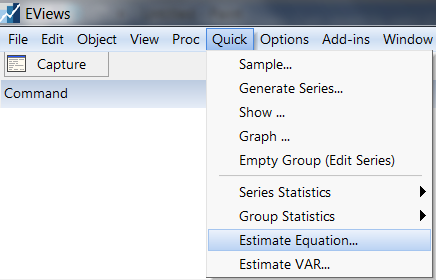
\includegraphics{esteqn}
		\end{figure}
		\vspace{-\baselineskip}
		\noindent then in the \textit{Equation Estimation} windows type in,
		$$deaths\ c\ alcohol$$
		\begin{figure}[H]
			\centering
			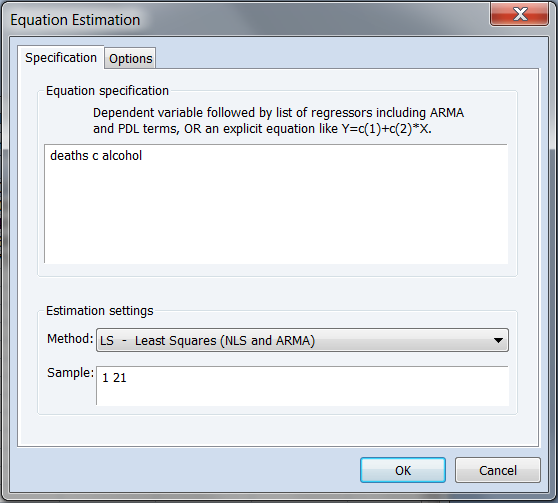
\includegraphics{esteqn1}
		\end{figure}
		\vspace{-\baselineskip}		
		%%%%%%%%%% TABLE OBJECT %%%%%%%%%%
		\begin{table}[H]
			\centering
			\begin{tabular}{lrrrr}
				\multicolumn{3}{l}{Dependent Variable: DEATHS}&\multicolumn{1}{c}{}&\multicolumn{1}{c}{}\\
				\multicolumn{3}{l}{Method: Least Squares}&\multicolumn{1}{c}{}&\multicolumn{1}{c}{}\\
				\multicolumn{2}{l}{Sample: 1 21}&\multicolumn{1}{c}{}&\multicolumn{1}{c}{}&\multicolumn{1}{c}{}\\
				\multicolumn{3}{l}{Included observations: 21}&\multicolumn{1}{c}{}&\multicolumn{1}{c}{}\\
				[4.5pt] \hline \\ [-4.5pt]
				\multicolumn{1}{c}{Variable}&\multicolumn{1}{r}{Coefficient}&\multicolumn{1}{r}{Std. Error}&\multicolumn{1}{r}{t-Statistic}&\multicolumn{1}{r}{Prob.}\\
				[4.5pt] \hline \\ [-4.5pt]
				\multicolumn{1}{c}{C}&\multicolumn{1}{r}{$876.2050$}&\multicolumn{1}{r}{$30.46816$}&\multicolumn{1}{r}{$28.75805$}&\multicolumn{1}{r}{$0.0000$}\\
				\multicolumn{1}{c}{ALCOHOL}&\multicolumn{1}{r}{$-16.26352$}&\multicolumn{1}{r}{$8.198924$}&\multicolumn{1}{r}{$-1.983616$}&\multicolumn{1}{r}{$0.0619$}\\
				[4.5pt] \hline \\ [-4.5pt]
				\multicolumn{1}{l}{R-squared}&\multicolumn{1}{r}{$0.171562$}&\multicolumn{2}{l}{Mean dependent var}&\multicolumn{1}{r}{$830.0476$}\\
				\multicolumn{1}{l}{Adjusted R-squared}&\multicolumn{1}{r}{$0.127960$}&\multicolumn{2}{l}{S.D. dependent var}&\multicolumn{1}{r}{$96.51864$}\\
				\multicolumn{1}{l}{S.E. of regression}&\multicolumn{1}{r}{$90.13207$}&\multicolumn{2}{l}{Akaike info criterion}&\multicolumn{1}{r}{$11.93082$}\\
				\multicolumn{1}{l}{Sum squared resid}&\multicolumn{1}{r}{$154352.0$}&\multicolumn{2}{l}{Schwarz criterion}&\multicolumn{1}{r}{$12.03030$}\\
				\multicolumn{1}{l}{Log likelihood}&\multicolumn{1}{r}{$-123.2736$}&\multicolumn{2}{l}{Hannan-Quinn criter.}&\multicolumn{1}{r}{$11.95241$}\\
				\multicolumn{1}{l}{F-statistic}&\multicolumn{1}{r}{$3.934731$}&\multicolumn{2}{l}{Durbin-Watson stat}&\multicolumn{1}{r}{$1.964148$}\\
				\multicolumn{1}{l}{Prob(F-statistic)}&\multicolumn{1}{r}{$0.061939$}&\multicolumn{1}{c}{}&\multicolumn{1}{c}{}&\multicolumn{1}{c}{}\\
				[4.5pt] \hline \\ [-4.5pt]
			\end{tabular}
			\caption{Regression output of $deaths$ on a constant and $alcohol$}
			\label{tbl:regout1}
		\end{table}
		\vspace{-\baselineskip}
		\noindent We report the estimated model by placing a `hat' above the dependent variable and the standard error of the estimated coefficient in parenthesis underneath the estimated coefficient,
		$$\widehat{deaths}_i = \underset{(30.4682)}{876.2050}-\underset{(8.1989)}{16.2635}alcohol_i$$
		$$i = 1, 2, \dots, 21$$
		\noindent To name/save this regression output into our workfile,
		$$Name \to Name\ to\ indentify\ object:eq01 \to OK$$
		\begin{figure}[H]
			\centering
			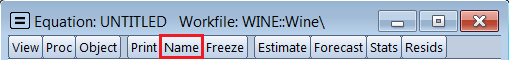
\includegraphics{esteqn3}
		\end{figure}
		\vspace{-\baselineskip}
		\begin{figure}[H]
			\centering
			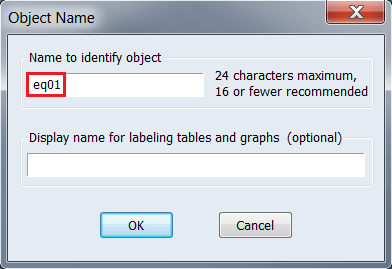
\includegraphics{esteqn4}
		\end{figure}
		\vspace{-\baselineskip}
	\newpage	
	\section*{Question 5}
	\underline{Predictive analytics}
	
		\noindent So far, we have generated outputs in EViews by `pointing-and-clicking'. We can also obtain these outputs by executing lines of code through the \textbf{Command} window,
		\begin{figure}[H]
			\centering
			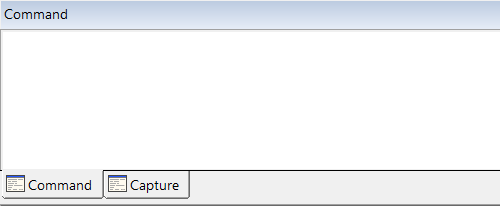
\includegraphics{cmdwin}
		\end{figure}
		\vspace{-\baselineskip}
		\noindent The Command window can also functions as a calculator. For example, we can use our estimated regression model,
		$$\widehat{deaths}_i = \underset{(30.4682)}{876.2050}-\underset{(8.1989)}{16.2635}alcohol_i$$
		$$i = 1, 2, \dots, 21$$
		\noindent to calculate the number of death per 100,000 of the population for a country that consumes \underline{3} litres of wine per capita per annum,
		$$\widehat{deaths} = 876.2050 - 16.2635\times3$$ This is an example of predictive analytics. We have estimated a regression model of $deaths$ and used this model to predict the number of death per 100,000 when a country consumes 3 litres of wine per capita per annum.
		
		\noindent From the Command window, executing the code
		$$scalar\ prediction=c(1)+c(2)^*3$$
		will store the calculation into a \textbf{scalar} object named \textit{prediction}.
		\begin{figure}[H]
			\centering
			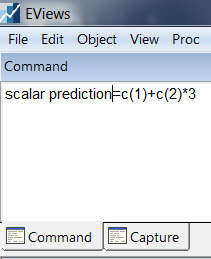
\includegraphics{pred1}
		\end{figure}
		\vspace{-\baselineskip}
		\noindent Note: $c(1)$ and $c(2)$ represents the $1^{st}$ and $2^{nd}$ estimated coefficient of the \underline{most recent} estimated regression model i.e. the values $876.2050$ and $-16.2635$
		
		\begin{figure}[H]
			\centering
			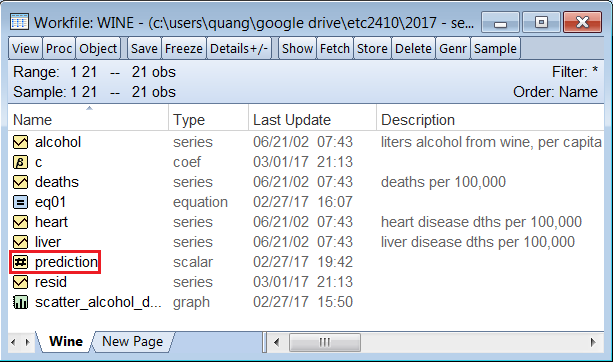
\includegraphics{pred2}
		\end{figure}
		\vspace{-\baselineskip}
		
	\section*{Question 6}
	\underline{Presenting results} \par
		\noindent (discuss in class)
	
	\section*{Question 7}
		\noindent Discuss each of the outputs you obtained above. What do you learn about the impact of alcohol consumption on the death rate? How could you improve your analysis?
		
		\noindent (discuss in class)
		
\end{document}